\documentclass[dvipdfm]{beamer}

\usepackage{bm}
\usepackage{helvet}
\usepackage{listings}
\lstset{
  language={python},
  basicstyle={\ttfamily\tiny},
  keywordstyle={\color{blue}},
  commentstyle={\color{green}},
  stringstyle=\color{red},
  tabsize=2,
  breaklines=true,
}

\usetheme{Madrid}
\usecolortheme{crane}
\setbeamercolor{structure}{fg=orange}
\setbeamercolor{block title example}{fg=white}
\setbeamercolor{block title alerted}{fg=white}
\setbeamertemplate{navigation symbols}{}
\setbeamertemplate{blocks}[rounded][shadow=false]
\setbeamertemplate{items}[circle]
\renewcommand{\kanjifamilydefault}{\gtdefault}
\usefonttheme[onlymath]{serif}
\renewcommand{\figurename}{図}
\renewcommand{\tablename}{表}
\renewcommand{\footnoterule}{
  \hrule width \textwidth height 0.5pt
  \kern 4pt
}

\title[研究会]{
    学習済みtransformerモデルのコンテキスト拡張 \\
    における位置エンコーディング
}
\subtitle[]{情報数理システム分野 研究会}
\author[平田 蓮]{平田 蓮}
\date{2024年5月22日}

\begin{document}
    \begin{frame}
        \titlepage
    \end{frame}
    \begin{frame}{Attention機構}
        \begin{block}{Attention機構}
            入力トークンの特徴量を、
            他トークンとの「関係性」を加味しながら計算する仕組み

            最終的なトークンの特徴量は、Attention機構を繰り返し通すことで形成される
        \end{block}
    \end{frame}
    \begin{frame}{Attention機構}
        各Attention機構では、前の段階で作られた特徴量からトークンごとに
        線形層を用いてQuery, Key, Valueの三種類のベクトルを構成する

        \begin{figure}
            \centering
            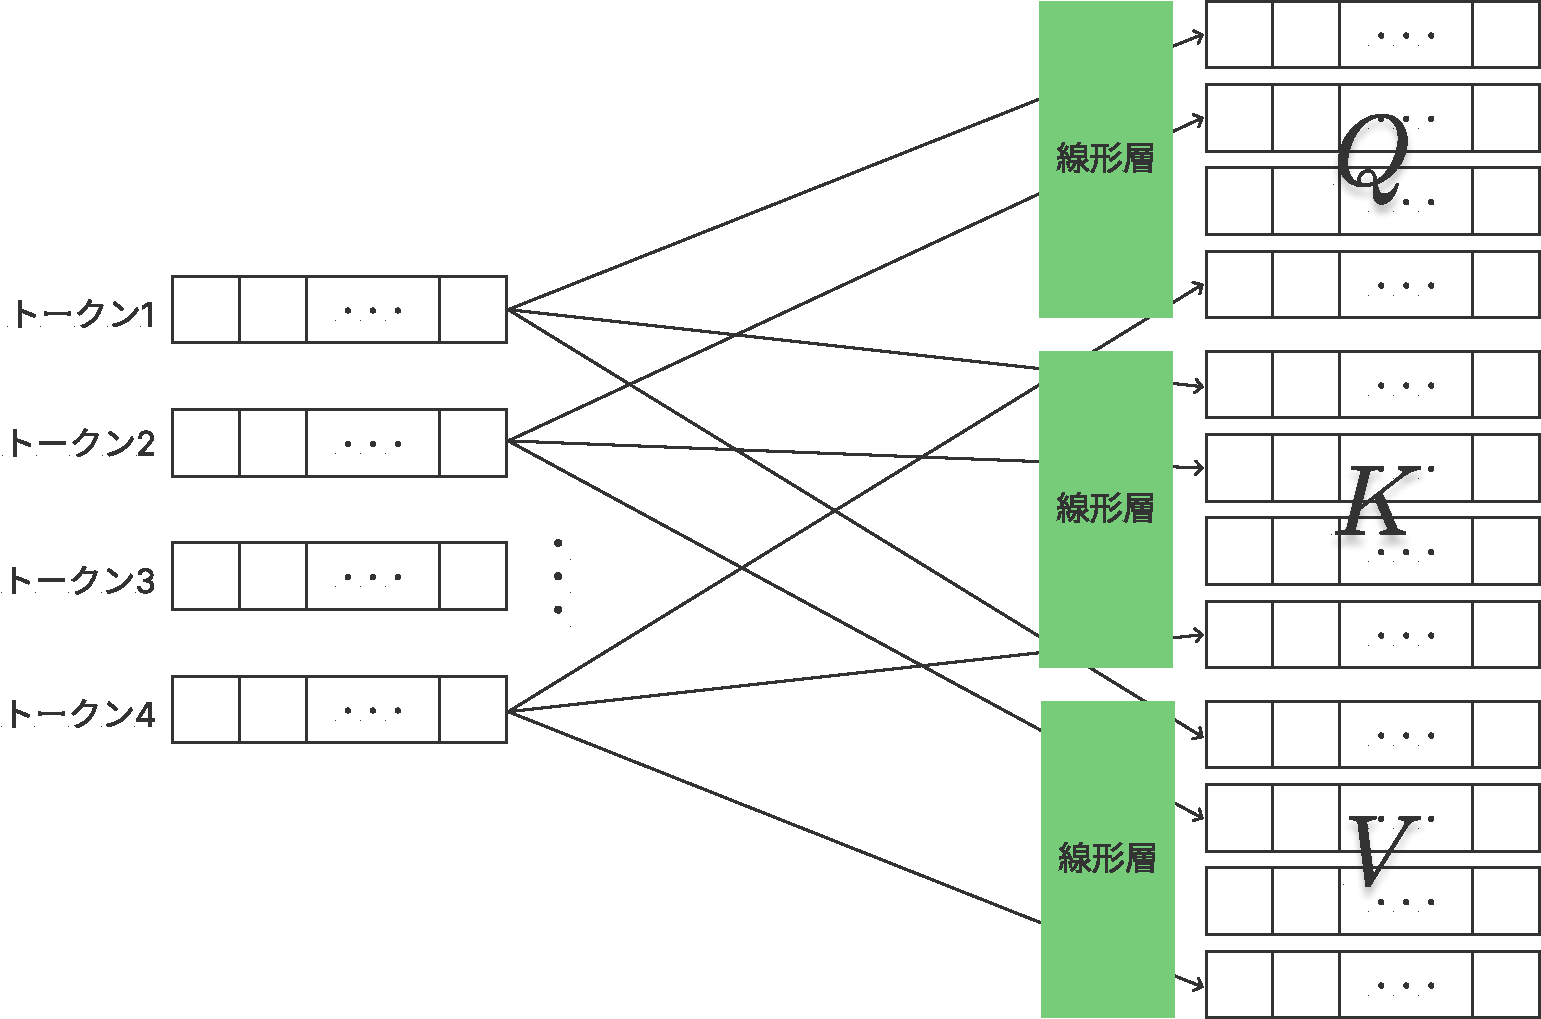
\includegraphics[width=.6\hsize]{qkv.pdf}
        \end{figure}
    \end{frame}
    \begin{frame}{Attention機構}
        それぞれのベクトルの意味のイメージは次の通り
        \begin{block}{}
            \begin{description}
                \item[Query] 自身のトークンと関連性の強いトークンを参照する
                \item[Key] 各トークンのQueryに対して適切な自身のValueを返す
                \item[Value] トークンの「値」
            \end{description}
        \end{block}
    \end{frame}
    \begin{frame}{Attention機構}
        $Q, K$を用いて次の式に基づいてAttention行列$A$を計算する
        \begin{align*}
            A = \mathrm{Softmax}\left(\frac{Q^t\!K}{\sqrt{d}}\right)
        \end{align*}

        \begin{figure}
            \centering
            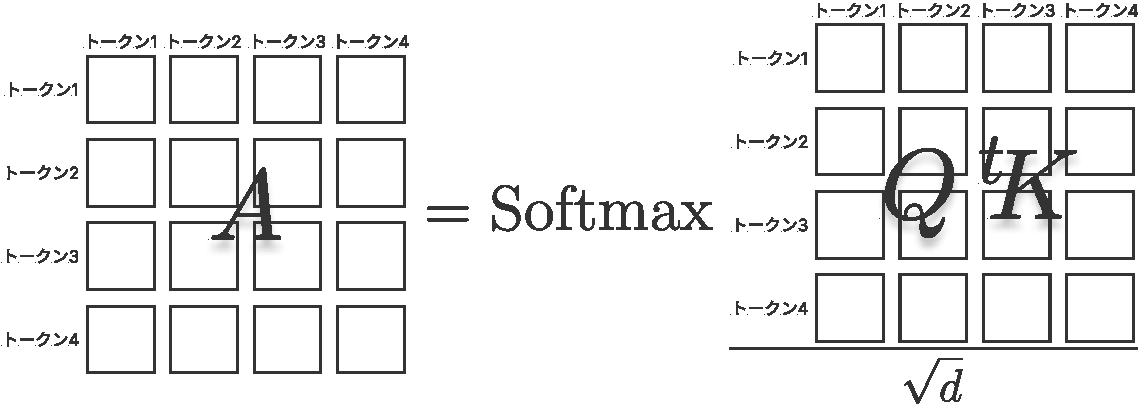
\includegraphics[width=.8\hsize]{attention1.pdf}
        \end{figure}
        $Q$と$K$を掛けることで各トークン同士の関係の強さを計算し、
        それを正規化したものが$A$である
    \end{frame}
    \begin{frame}{Attention機構}
        $A$を計算した後、
        $AV$の各行が各トークンの特徴量として次のAttention機構に渡される

        \begin{figure}
            \centering
            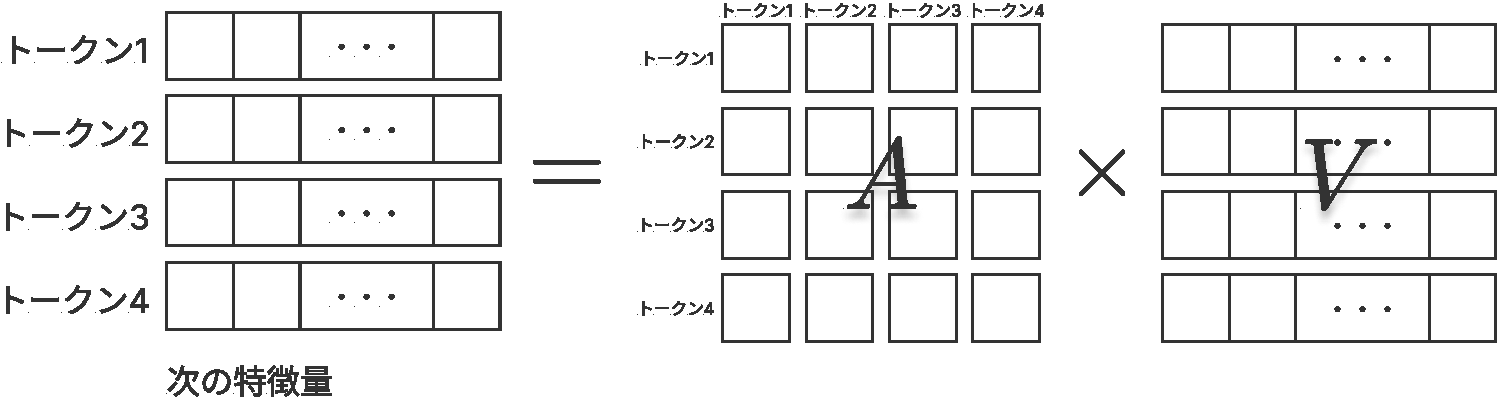
\includegraphics[width=1\hsize]{attention2.pdf}
        \end{figure}
    \end{frame}
    \begin{frame}{位置エンコーディング}
        \begin{block}{Attention機構の問題点}
            トークンの順番を入れ替えても同様の特徴量が得られてしまうという問題がある。
            よって、上述のように計算をするとトークン同士の位置情報が失われる。
        \end{block}
        
        この問題を解消するため、$A$を計算する際に位置情報を加味した計算を追加で行う。
        これを\structure{位置エンコーディング}と呼ぶ。
    \end{frame}
    \begin{frame}{位置エンコーディング - 絶対位置エンコーディング}
        次の式で計算されるベクトルを各トークンの特徴量に加算する
        \begin{block}{}
            \begin{align*}
                \mathrm{Positional Encoding} = \left\{
                    \begin{aligned}
                        & \sin\left(\frac{i}{10000^{\frac{2j}{d}}}\right) \ (j\equiv 0 \mod 2) \\
                        & \cos\left(\frac{i}{10000^{\frac{2j}{d}}}\right) \ (j\equiv 1 \mod 2)
                    \end{aligned}
                    \right.
            \end{align*}

            \begin{description}
                \item[$i$] トークンの位置
                \item[$j$] 位置エンコーディングの要素の位置
            \end{description}
        \end{block}
    \end{frame}
    \begin{frame}{位置エンコーディング - 相対位置エンコーディング}
        絶対位置エンコーディングの改善点1
        \begin{exampleblock}{時系列データは絶対位置よりも、他のトークンとの相対位置が重要}
            日本語の文章で考えると、
            「私のペンが…」と「〇〇。私のペンが…」という2つのシーケンスでは
            「ペン」の位置が違うので絶対位置エンコーディングでは別の値となるが、
            実際は「私の」の次にあるという相対的な位置情報が大事である
        \end{exampleblock}
    \end{frame}
    \begin{frame}{位置エンコーディング - 相対位置エンコーディング}
        絶対位置エンコーディングの改善点2
        \begin{exampleblock}{学習データに無い長さの系列を処理できない}
            学習データに無い長さの系列をモデルに与えた時、
            後ろの方の絶対位置エンコーディングは学習されていない状態であるため、
            適切な推論ができなくなることが確認されている
            
        \end{exampleblock}
        \begin{figure}[h]
            \centering
            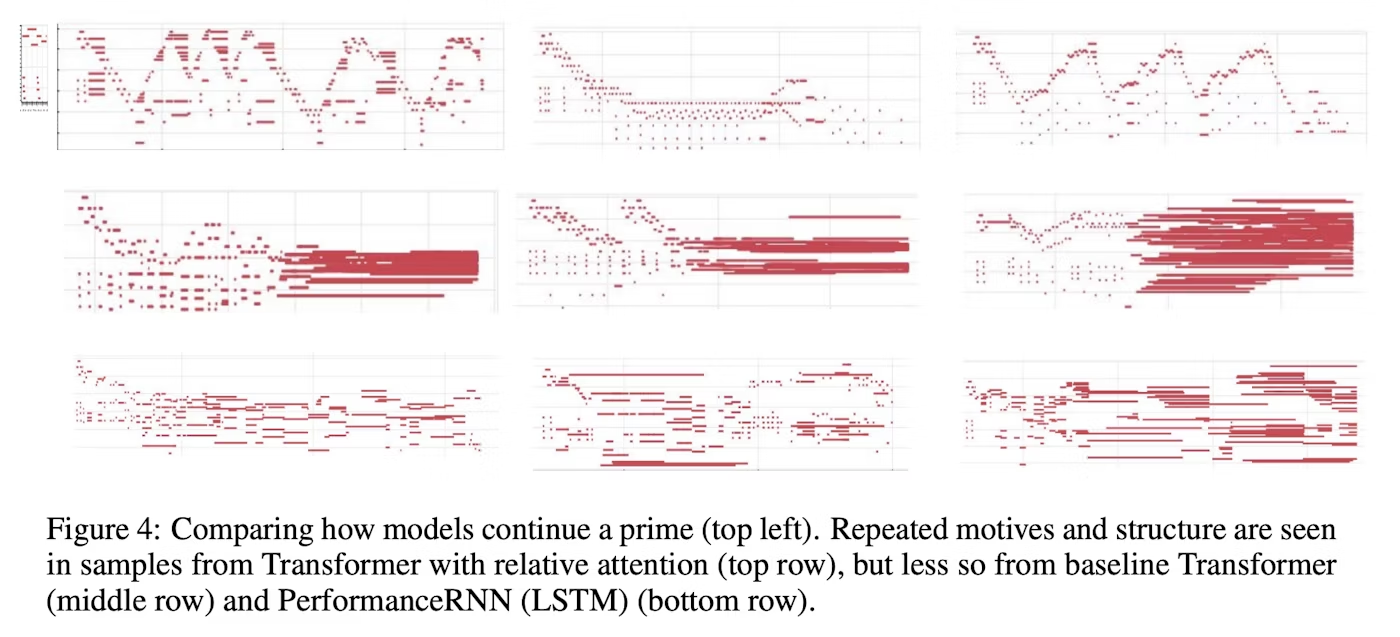
\includegraphics[width=.8\linewidth]{catastrophie.png}
        \end{figure}
    \end{frame}
    \begin{frame}{位置エンコーディング - 相対位置エンコーディング}
        相対位置エンコーディングは下図に示すような行列であり、
        Attention行列を計算する際に$Q^t\!K$に加算される。
        \begin{figure}[h]
            \centering
            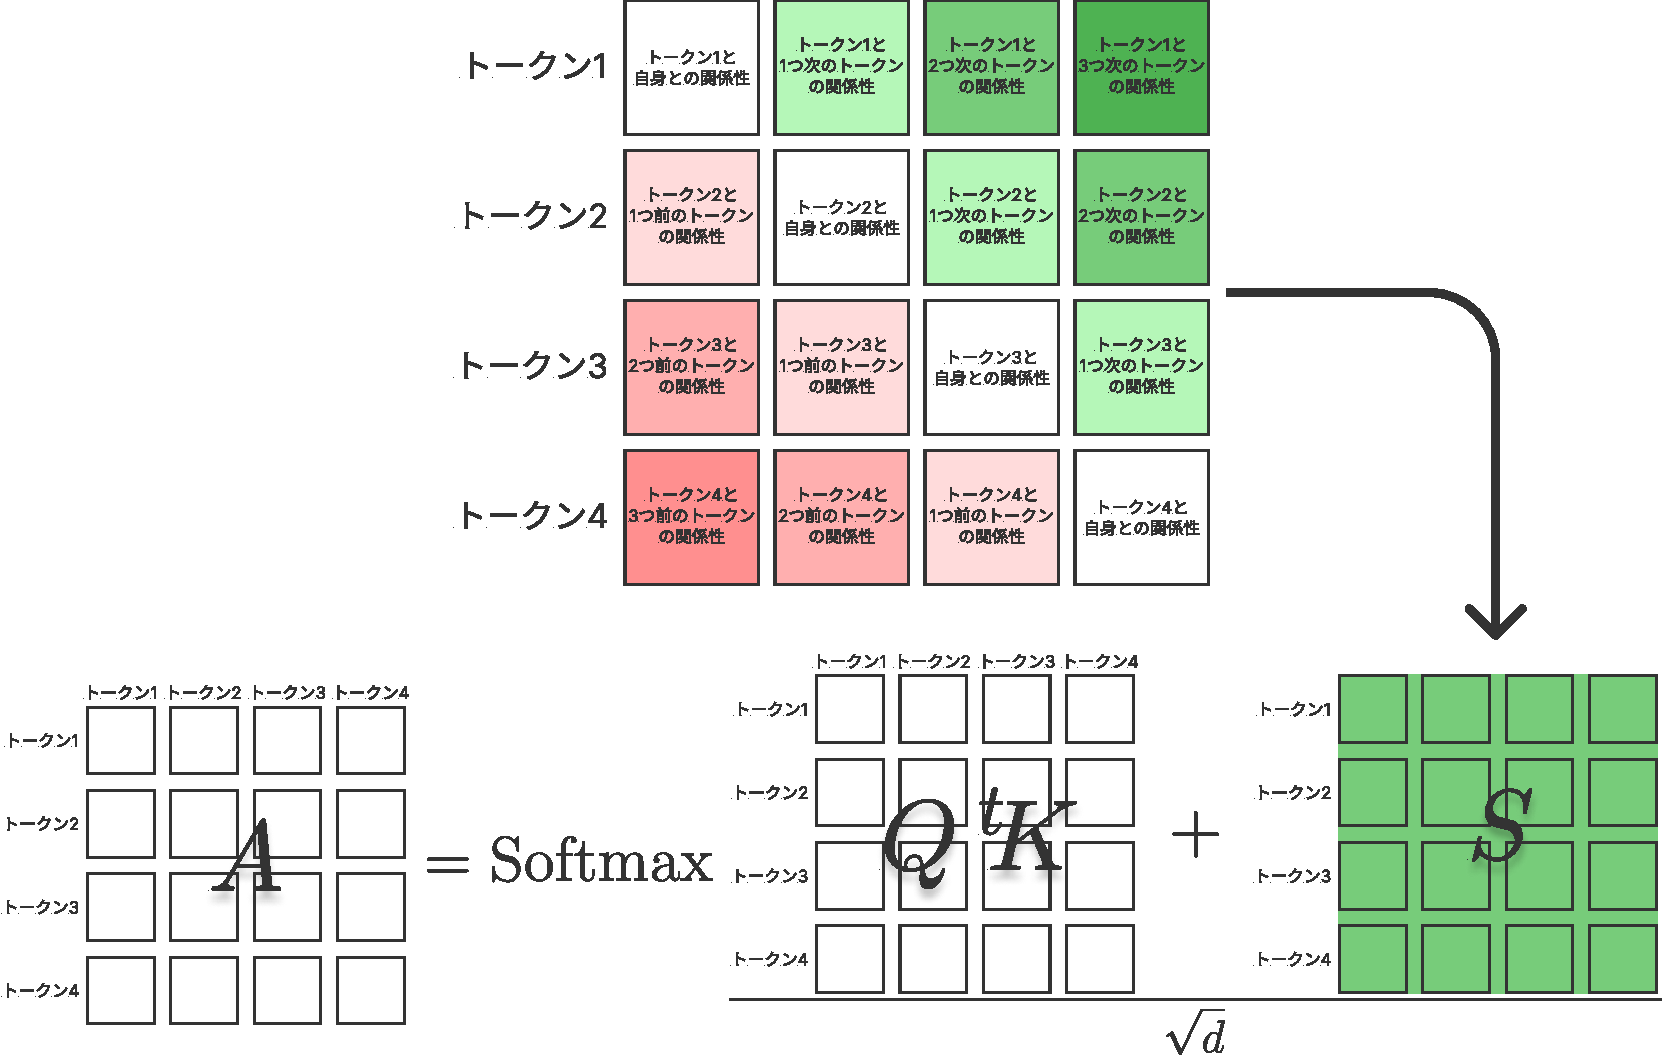
\includegraphics[width=.8\linewidth]{relative.pdf}
        \end{figure}
    \end{frame}
    \begin{frame}{位置エンコーディング - 相対位置エンコーディング}
        相対位置エンコーディングの行列は、
        各Attention機構が固有に保持する相対位置ごとの埋め込みと、
        各トークンのQueryの内積で計算される。
        \begin{block}{}
            \begin{align*}
                S_{i,j} = Q_iE_{i-j}
            \end{align*}

            \begin{description}
                \item[$S_{i,j}$] $S$の$(i,j)$要素
                \item[$Q_i$] $i$番目のトークンのQuery
                \item[$E_{i-j}$] {
                    あるトークンとそれから$i-j$の位置との相対位置埋め込み。
                    \structure{学習可能パラメータ}
                }
            \end{description}
        \end{block}
    \end{frame}
    \begin{frame}{位置エンコーディング - RoPE}
        位置エンコーディングを加算ではなく乗算で行うアプローチ。
        LLaMAなどで用いられており、現在主流である。

        QueryとKeyに回転行列をかけて、ベクトルを回転させることで位置情報を乗せる。

        \begin{block}{RoPEの特徴}
            \begin{itemize}
                \item トークンの位置ごとに回転角を増やしていくため、絶対位置情報を反映可能
                \item 距離の近いトークンの回転角同士が成す角が小さいため、相対位置情報も反映可能
            \end{itemize}
        \end{block}
    \end{frame}
    \begin{frame}{位置エンコーディング - RoPE}
        \begin{block}{回転行列の計算}
            {\small
                \begin{align*}
                    R &= \begin{pmatrix}
                        \cos m\theta_1 & -\sin m\theta_1 & 0 & 0 & \cdots & 0 & 0 \\
                        \sin m\theta_1 & \cos m\theta_1 & 0 & 0 & \cdots & 0 & 0 \\
                        0 & 0 & \cos m\theta_2 & -\sin m\theta_2 & \cdots & 0 & 0 \\
                        0 & 0 & \sin m\theta_2 & \cos m\theta_2 & \cdots & 0 & 0 \\
                        \vdots & \vdots & \vdots & \vdots & \ddots & \vdots & \vdots \\
                        0 & 0 & 0 & 0 & \cdots & \cos m\theta_\frac{d}{2} & -\sin m\theta_\frac{d}{2} \\
                        0 & 0 & 0 & 0 & \cdots & \sin m\theta_\frac{d}{2} & \cos m\theta_\frac{d}{2}
                    \end{pmatrix} \\
                    \theta_i &= 10000^{-\frac{2(i-1)}{d}} \ \left(i = 1, 2, \cdots, \frac{d}{2}\right)
                \end{align*}
            }

            \begin{description}
                \item[$m$] トークン位置
            \end{description}
        \end{block}
        これを用いて計算した$^t\!Q' = R^t\!Q, ^t\!K' = R^t\!K$により
        Attention行列を計算する。
    \end{frame}
    \begin{frame}{コンテキスト拡張}
        現在、学習済みのモデルのコンテキストを拡張する際の位置エンコーディングは、
        Scaled RoPEが主流に用いられている
        \begin{block}{Scaled RoPE}
            RoPEをコンテキスト長の拡張に応じて引き伸ばす手法

            上述の$m$を元のコンテキスト長$n$と
            新しいコンテキスト長$n'$を用いて$\displaystyle\frac{n}{n'}$倍する。
        \end{block}
    \end{frame}
    \begin{frame}{展望 - 別アプローチによる位置エンコーディングの拡張}
        \begin{alertblock}{Scaled Ropeの問題点}
            コンテキスト長を大きくした際に位置エンコーディングの「差」が小さくなってしまうため、
            極端にコンテキスト長を長くした際に位置エンコーディングの意味が薄れてしまう
        \end{alertblock}
        これを回避した\structure{再学習あり}のコンテキスト拡張の手法も提案されているが、
        学習済みの位置エンコーディングを拡張する手法は見つけられていないため、
        調査を継続したい。
    \end{frame}
    \begin{frame}{展望 - 位置エンコーディングのスパース性}
        gpt-3の埋め込み次元は3072, 最大トークン長は8192である
        \footnote{https://platform.openai.com/docs/guides/embeddings/what-are-embeddings}。
        このときの絶対位置エンコーディングとRoPEの具体的な値を見てみる。
    \end{frame}
    \begin{frame}{展望 - 位置エンコーディングのスパース性}
        \begin{figure}
            \centering
            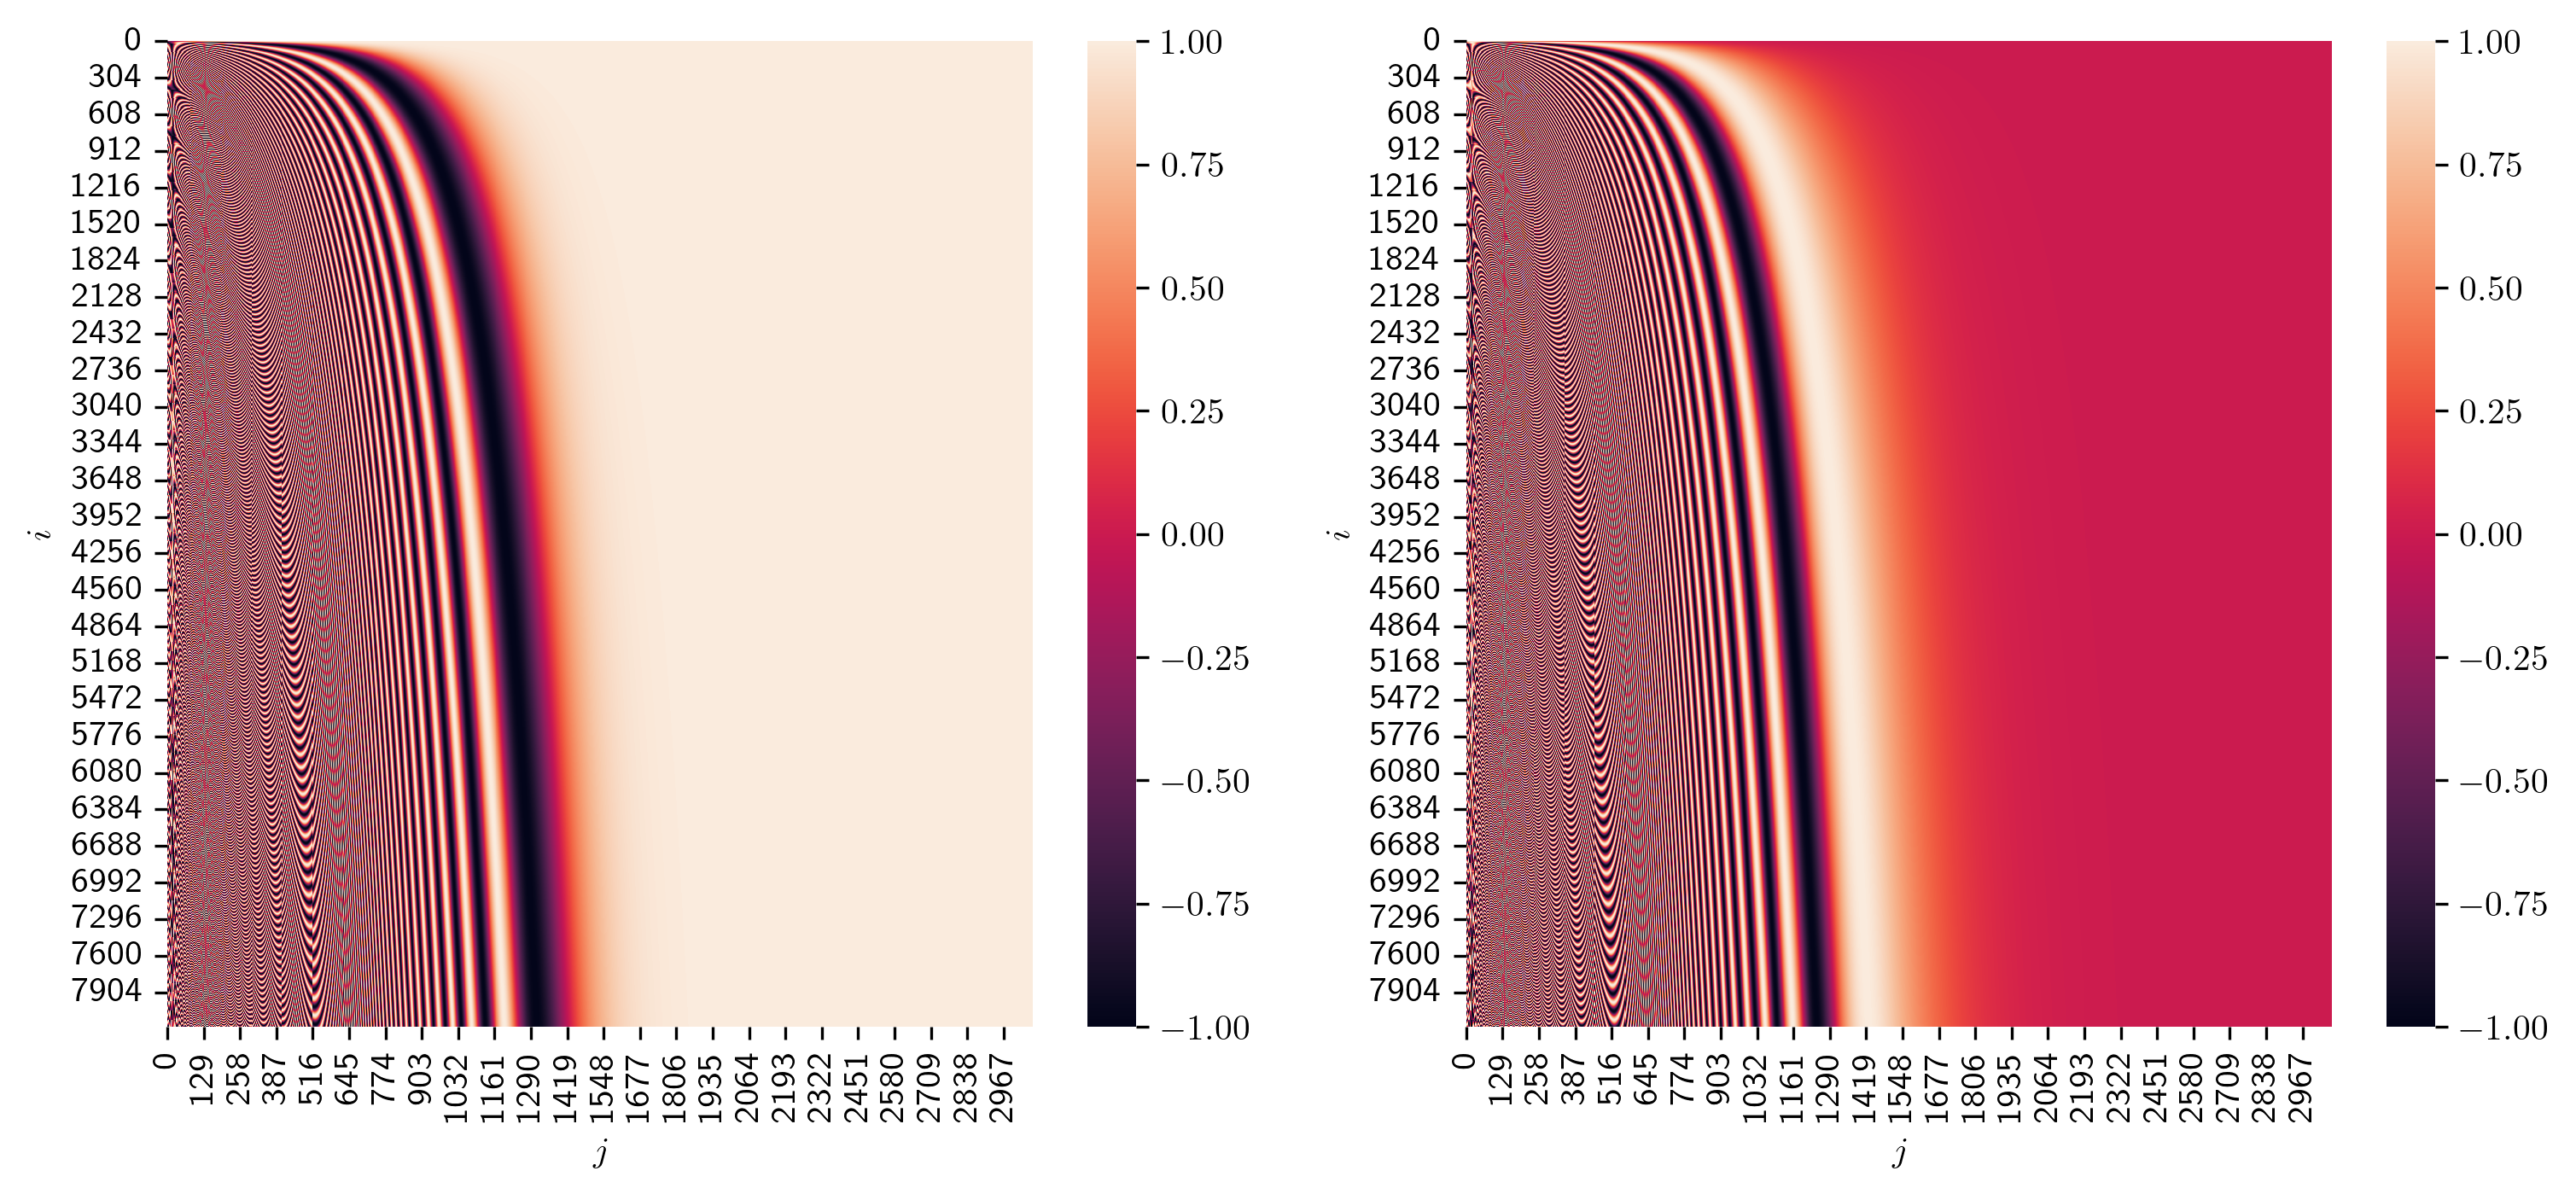
\includegraphics[width=1\linewidth]{absolute.png}
            \caption{
                絶対位置エンコーディングの値。
                $\cos$(左)と$\sin$(右)。
            }
        \end{figure}
    \end{frame}
    \begin{frame}{展望 - 位置エンコーディングのスパース性}
        \begin{figure}
            \centering
            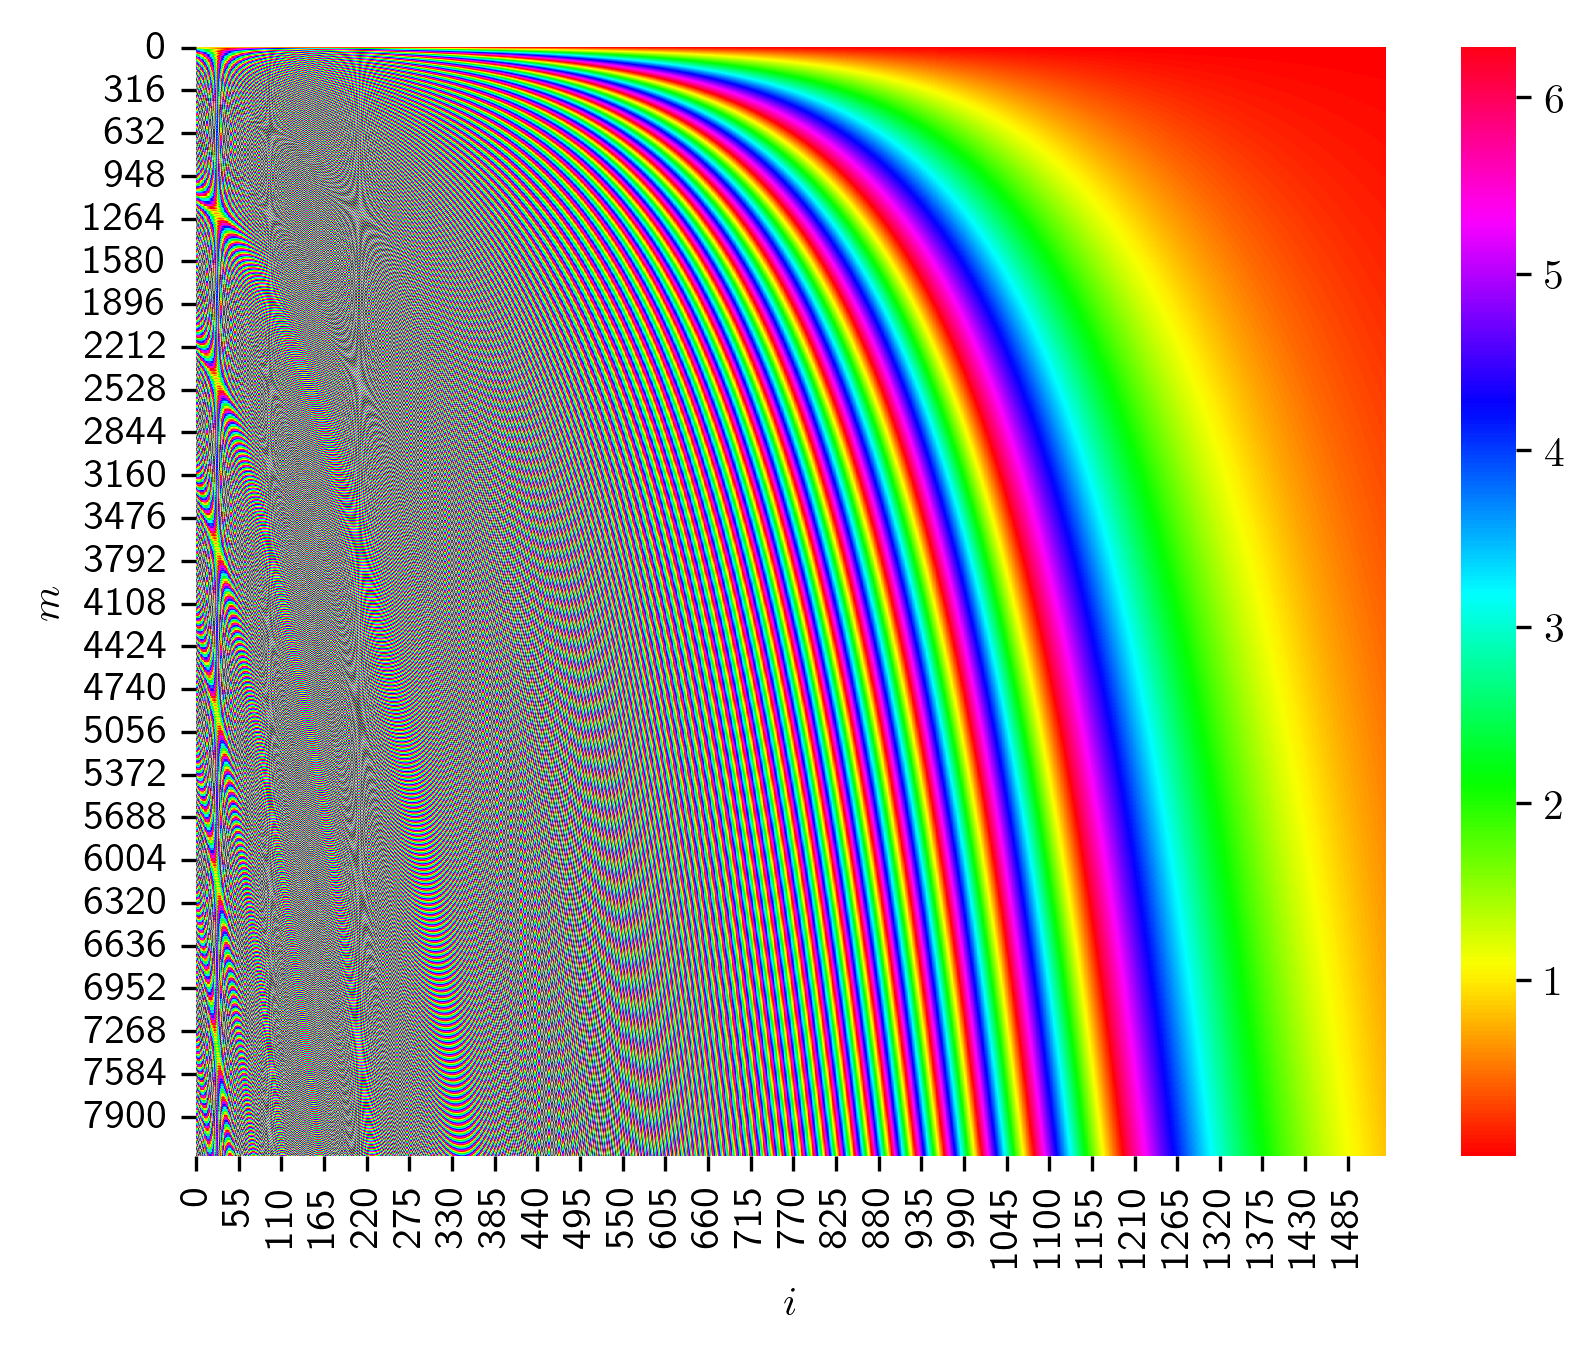
\includegraphics[width=0.6\linewidth]{rope.png}
            \caption{
                RoPEのの回転角$m\theta_i$
            }
        \end{figure}
    \end{frame}
    \begin{frame}{展望 - 位置エンコーディングのスパース性}
        図を見ると、各ベクトルにおいて、
        高次元の部分には位置エンコーディングの情報が乗っていないことがわかる。
        これを踏まえると、
        次の二つの可能性を感じるため、調査を続けたい。
        \begin{block}{位置エンコーディングの情報量を増やして性能が向上する場合}
            よりベクトル全体に情報を乗せる「効率的」な位置エンコーディング
        \end{block}
        \begin{block}{情報量が少ない位置エンコーディングで十分な場合}
            よりスパースな、計算量を削減できる位置エンコーディング
        \end{block}
    \end{frame}
\end{document}